Developing (and breaking) attentional habits: How extended training shifts decision making from rational to heuristic.

Omar David Perez\textsuperscript{1,3}, Sebastian Muñoz\textsuperscript{1}, \& Bastian Henriquez-Jara\textsuperscript{2,3}

\textsuperscript{1} Department of Industrial Engineering, University of Chile, Santiago, Chile.

\textsuperscript{2} Department of Civil Engineering, University of Chile, Santiago, Chile.

\textsuperscript{3} Instituto Sistemas Complejos de Ingeniería (ISCI), Chile.

Author Note

Correspondence regarding this article should be sent to Omar D. Perez (\href{mailto:omar.perez.r@uchile.cl}{\ul{omar.perez.r@uchile.cl}}) or Bastian Henriquez-Jara (\href{mailto:bastian.henriquez@ug.uchile.cl}{\ul{bastian.henriquez@ug.uchile.cl}}).

\section{}\label{section}

\section{Abstract}\label{abstract}

Habits are fixed behavioral patterns formed through repetition in stable environments and are typically insensitive to changes in outcome value. In this study, we propose that attention itself may become habitual---narrowing over time and leading to stereotyped sampling of information. Using eye-tracking in a discrete-choice experiment with over 150 trials, we show that participants progressively subsample outcome attributes, reducing the diversity of information considered. This attentional narrowing mirrors the rigidity and stereotypical patterns observed in habitual behavior. However, we also demonstrate that simple contextual manipulations---such as altering the spatial layout of options---can restore goal-directed attention. Computational modeling reveals that these attentional patterns significantly modulate estimated preferences, linking attentional focus to value construction and choices. These findings position attention as a dynamic and experience-sensitive mechanism, offering insight into the cognitive processes underlying both the formation and disruption of habitual choices, and raising implications for models of decision-making that assume stable preferences and information processing.

\emph{Keywords: habits, attention, discrete-choice, eye-tracking}

Developing (and breaking) attentional habits: an experimental study

\section{Introduction}\label{introduction}

A large body of work, both in animals and humans, shows that a behavior that is initially goal-directed, that is, sensitive to the causal association between behavior and its consequences, may turn into a habit when individuals make decisions repeatedly under stable conditions. Behavioral assays of habits demonstrate that when subjects enter into this habit or \emph{auto-pilot} mode, they become insensitive to changes in outcome value \href{https://www.zotero.org/google-docs/?vZFOZ6}{(Dickinson, 1985; Dolan \& Dayan, 2013; Perez \& Dickinson, 2020; Pool et al., 2022)}. For example, classic instrumental learning studies showed that rats trained for extended periods of time in a stable environment will continue to perform actions even when the outcomes are devalued and no longer satisfy their current needs and desires \href{https://www.zotero.org/google-docs/?ycvERy}{(Adams \& Dickinson, 1981)}. Similar studies in humans have shown that extended training across days progressively reduces sensitivity to outcome devaluation, especially in people that report higher levels of stress and anxiety \href{https://www.zotero.org/google-docs/?PJYiYt}{(Hardwick et al., 2019; Pool et al., 2022)}.

Recent studies in animals suggest that attention may be a critical factor linking stable environments to the development of habits \href{https://www.zotero.org/google-docs/?b2gFIo}{(Bouton et al., 2020; Thrailkill et al., 2018)}. In these studies, animals that are rewarded consistently in the presence of a discriminative stimulus---for example a light which signals the period in which responses may be reinforced---are more likely to develop habits compared to animals for which the stimulus only partially signals reinforcement, suggesting that habits emerge when animals are given extended training in a stable and predictable environment that leads them to stop paying attention to their behavior \href{https://www.zotero.org/google-docs/?nMgBaG}{(Bouton et al., 2020; Thrailkill et al., 2018)}. This line of research has also demonstrated that habits can be easily disrupted by changing the properties of the outcome after extended training, consistent with the idea that surprise and uncertainty may affect the attentional resources deployed for decision making \href{https://www.zotero.org/google-docs/?svzmKl}{(Daw et al., 2005; Lee et al., 2014)}, driving them to actions and their consequences and restore goal-directed control \href{https://www.zotero.org/google-docs/?I0feaJ}{(Bouton, 2024; Bouton et al., 2020)}. Habits, therefore, seem to be potentially breakable by manipulations of the environment.

In humans, there is recent evidence suggesting that attention may also play a role in habit formation. Inspired by commuting behavior in London underground users \href{https://www.zotero.org/google-docs/?jR8OZb}{(Larcom et al., 2017)} who showed a strong tendency to stick with familiar routes even when a strike that led to the closure of many stations force them to explore and discover better alternatives, Henriquez-Jara et al. (2025) trained participants in a simple computerized choice task between fictitious buses. Subjects first chose between two bus stops that led stochastically to two different buses which took them (also probabilistically) . Once participants had learned the better of these two, a third, objectively superior option was introduced. The key question was whether participants who initially behaved in line with model-free reinforcement learning (which is thought to capture habitual tendencies) would continue relying on the previously learned option, ignoring the better alternative. The results showed that model-free subjects were less likely to explore the new option compared to participants relying on goal-directed (model-based) strategies. Their results suggest that individuals prone to use habit-like strategies in their decisions focus attention on previously rewarded options, ignoring aspects of the environment (such as a new, better option) that may be beneficial.

In contrast with the psychological and neuroscience literature, human studies in decision-making have been studied largely in isolation from the literature on habits. Much of what we know in this area comes from work in economics, marketing and engineering using discrete-choice experiments (DCEs). In these experiments, subjects are presented with options that have different attribute values so that subjects have to weight each of them according to their preferences to make a choice, or else simple binary choice tasks (Krajbich et al., 2010; Bansal et al., 2024; Martinovici et al., 2023). These approaches have shown that attention can track attribute-level preferences and even predict eventual choices. But in contrast to the psychological literature, where attention is thought to play a role in habit formation, in these decision-making studies attention is usually treated as a stable mediator of preference expression---not as a process that evolves with experience. Indeed, because DCEs assume that preferences are stable and compensatory (i.e., all attributes are considered in a decision), attention is typically assumed to reflect those preferences consistently across time. As a result, little is known about how attention might change when individuals make repeated choices under stable conditions---the very conditions known to produce habitual behavior in psychology and neuroscience studies. The question of whether attention itself becomes habitual---narrowing to familiar cues and neglecting information about outcome value---remains largely unaddressed.

In this study, we propose that the formation of habits in humans may involve a progressive narrowing of attention: a ``habitual attention'' mechanism whereby participants begin to subsample the information, prioritizing a subset of attributes while ignoring others. Using eye-tracking in a large-scale discrete-choice experiment, we tracked how attention evolved as participants made repeated decisions across hundreds of trials, mimicking the overtraining manipulations employed in psychology and neuroscience. Our results reveal a systematic shift from broad, compensatory attention to a restricted, stereotyped sampling of attributes. This attentional shift mirrors the behavioral rigidity typically associated with habits---individuals stop encoding the full value of options and instead rely on a reduced and more automatic attentional strategy. Through computational modeling, we show that this attentional habit is reflected in preference and choice.

Critically, we also show that these attentional habits can be disrupted. A simple manipulation of the environment stability was sufficient to restore more exploratory patterns of attention that were again reflected in choices. When repeated across trials, the manipulation sustained this re-engagement, reducing inertia and promoting broader sampling of the environment. These findings suggest that attentional habits are not fixed: like behavior itself, they can be sensitive to contextual changes. Our results establish attention as a dynamic mechanism underlying habit formation---one that both reflects and shapes the transition from flexible, goal-directed control to stereotyped, habitual behavior.

\section{Results}\label{results}

The experiment was a discrete-choice task involving repeated decisions between three transportation modes (bus, metro, ride-hailing), each described by four attributes: cost, time, comfort, and CO₂ emissions (see Fig. 1). The study comprised 150 trials per participant, divided into two phases. In the Training phase (100 trials), participants made choices between the three options, with the context remaining stable. Colors and positions of rows (attribute labels) and columns (option labels) were fixed during this phase. In the Testing phase (50 trials), the position of attribute rows was shuffled every five trials with the aim of disrupting attentional habits and re-engage exploratory, goal-directed attention \href{https://www.zotero.org/google-docs/?wVg4TV}{(Dayan et al., 2000; Gottlieb, 2012)}. The values for each attribute in each trial were sampled through a widely-known algorithm in DCEs that ensured no alternative dominated the others (i.e., no alternative was objectively better than any other. See Methods section.)

Our analysis is divided in two sections. We first analyzed response times (RTs) and the correlation between attentional allocation and final choices, aiming to reproduce established findings from the literature. This involved assessing whether RTs decreased over trials, indicative of learning the structure of the task, and whether attentional patterns aligned with subsequent choices, as is usually observed in studies investigating the interplay between of attention on decision-making \href{https://www.zotero.org/google-docs/?broken=pHMYOR}{(Bansal et al., 2024; Krajbich et al., 2010; Krajbich \& Rangel, 2011; Martinovici et al., 2023)}. Our focus was on verifying basic experimental results from previous studies before delving into the more complex analyses of attentional habits. In the second section, we examined the evolution of attentional allocation over time, and how that evolution shapes final decisions. We focused on three key hypotheses: a) that participants would show more predictable patterns of attention as training progressed b) that attention span would change across training, fixating in some attributes over others c) that attention span and attribute switching would increase following the manipulation and c) that a computational model of decisions over trials would reflect the evolution of attentional span and strategies. Demographic variables were not included in the statistical models, as participants were assumed to be demographically homogeneous for the purposes of the present analysis (see Methods).

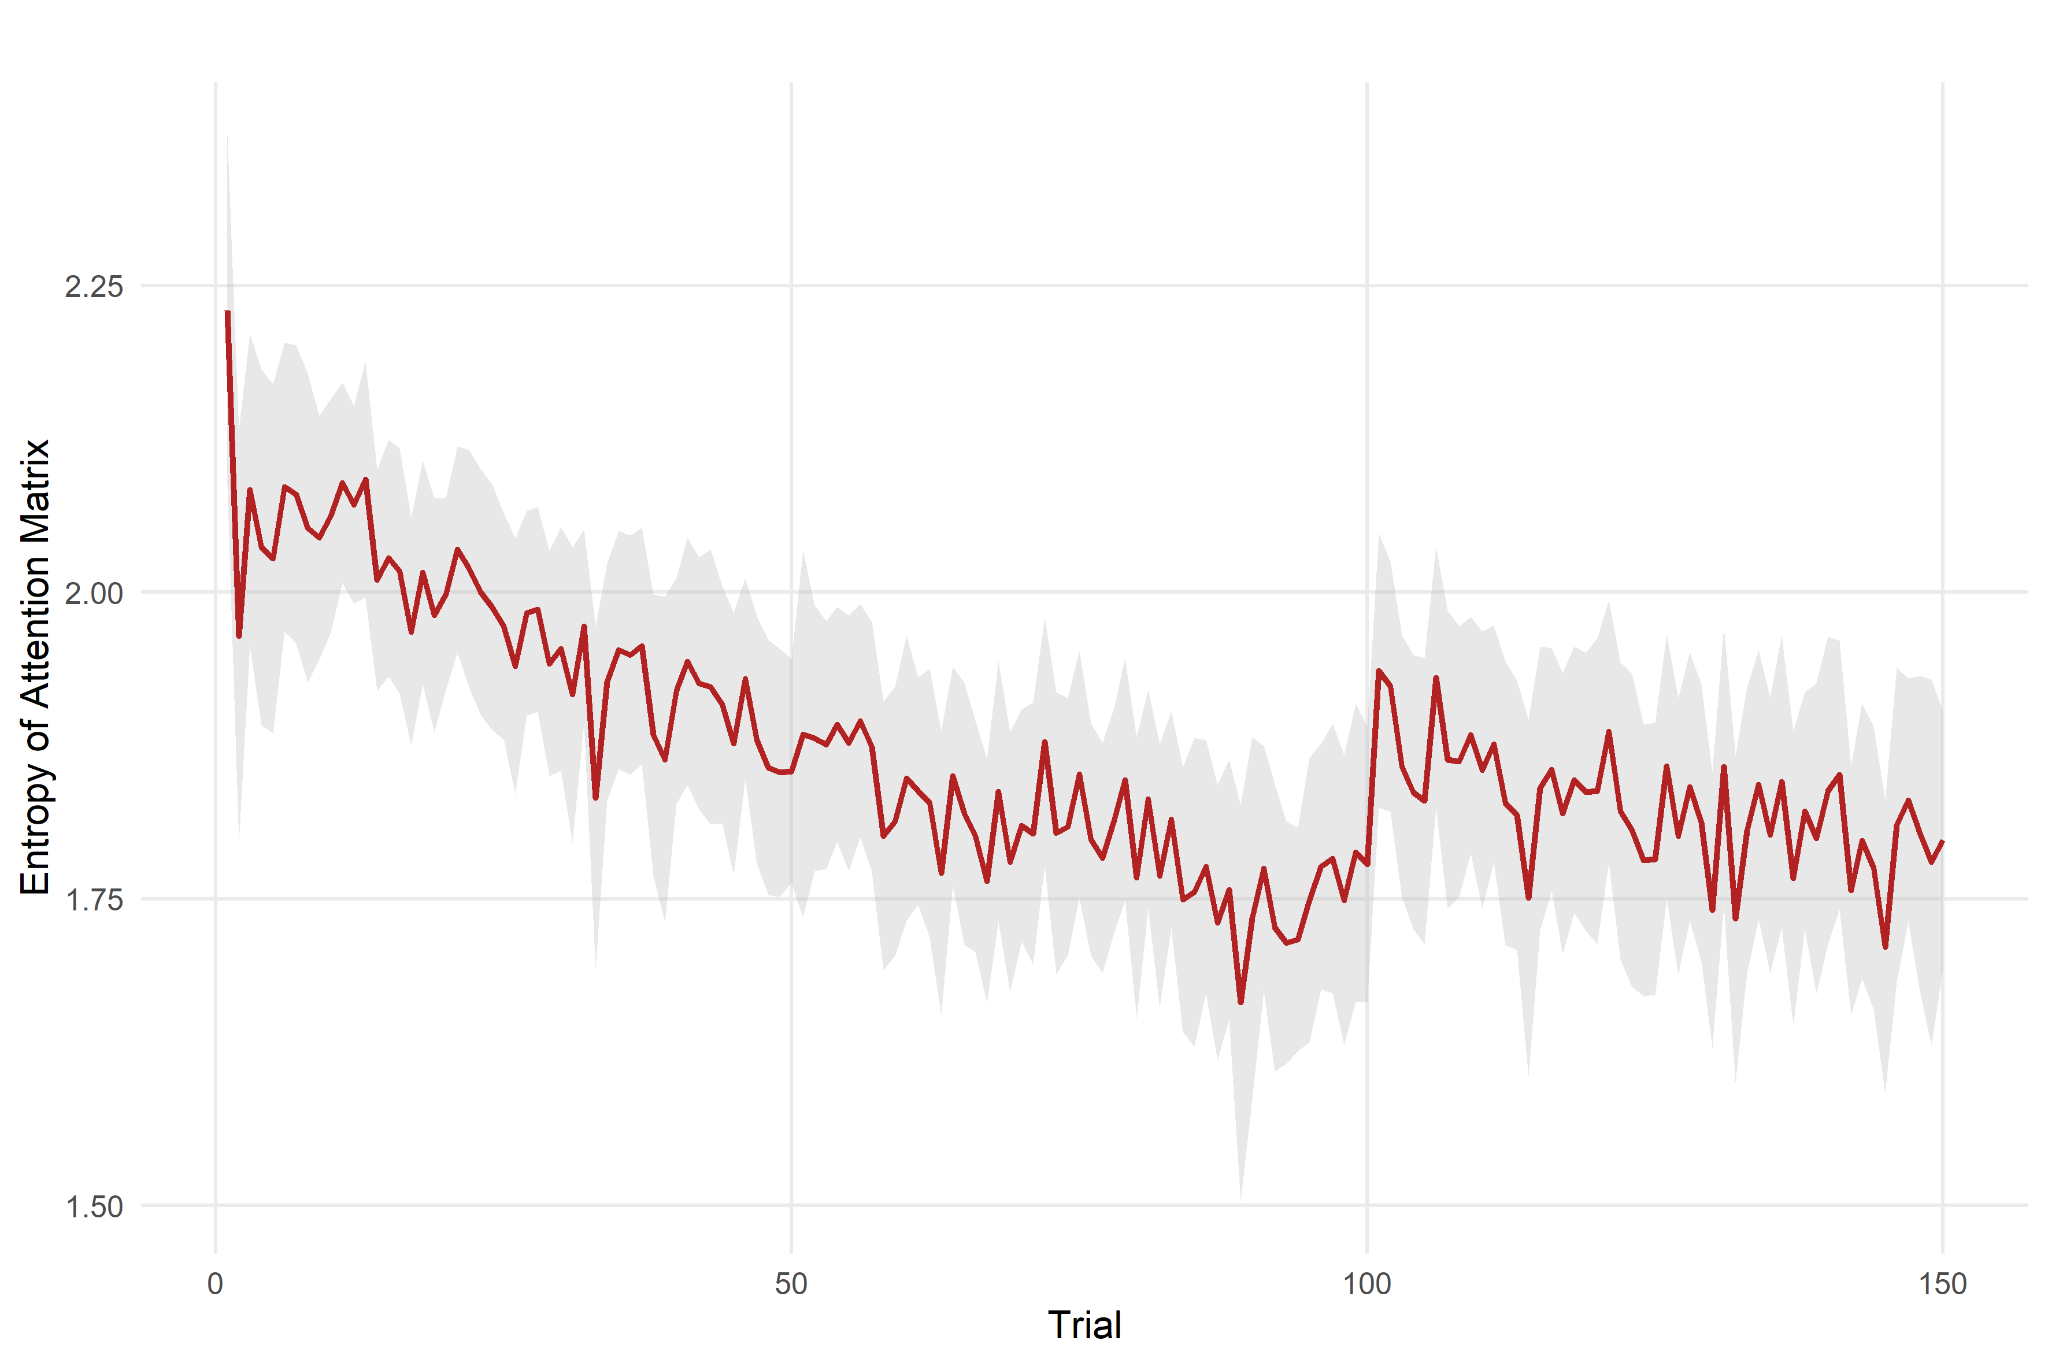
\includegraphics[width=4.06891in,height=2.70671in]{fig/word_media/media/image1.png}

{\def\LTcaptype{none} % do not increment counter
\begin{longtable}[]{@{}
  >{\raggedright\arraybackslash}p{(\linewidth - 6\tabcolsep) * \real{0.1961}}
  >{\raggedright\arraybackslash}p{(\linewidth - 6\tabcolsep) * \real{0.1881}}
  >{\raggedright\arraybackslash}p{(\linewidth - 6\tabcolsep) * \real{0.1865}}
  >{\raggedright\arraybackslash}p{(\linewidth - 6\tabcolsep) * \real{0.1881}}@{}}
\toprule\noalign{}
\endhead
\bottomrule\noalign{}
\endlastfoot
& Estimate & Std. Error & t value \\
(Intercept) & 2.070 & 0.042 & 49.786 \\
Trial & -0.004 & 0.000 & -28.264 \\
Manipulation & -0.003 & 0.046 & -0.067 \\
Trial x Manipulation & 0.002 & 0.000 & 4.347 \\
\end{longtable}
}

R2=0.586, fixed effect linear model (entropy\textasciitilde Trial*(Trial\textgreater100)+(1\textbar participant))

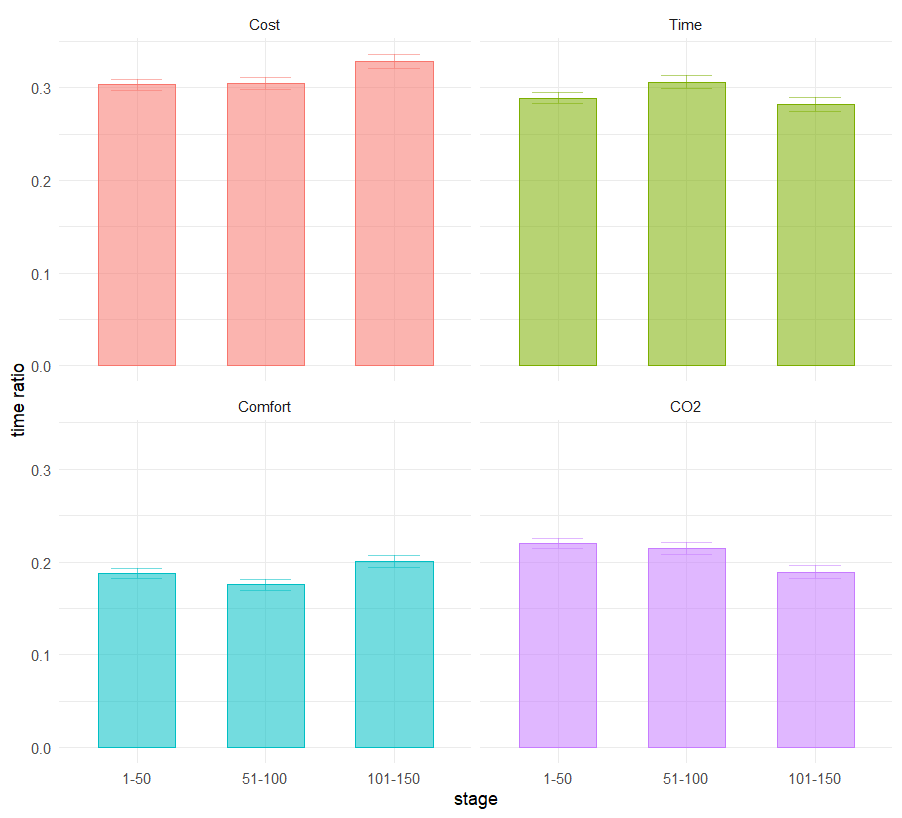
\includegraphics[width=6.18506in,height=5.60521in]{fig/word_media/media/image4.png}

Figure X. Fixation time ratio (Fixation time / trial time) by attribute, in 50-trials blocks.

{\def\LTcaptype{none} % do not increment counter
\begin{longtable}[]{@{}
  >{\raggedright\arraybackslash}p{(\linewidth - 6\tabcolsep) * \real{0.3971}}
  >{\raggedright\arraybackslash}p{(\linewidth - 6\tabcolsep) * \real{0.1559}}
  >{\raggedright\arraybackslash}p{(\linewidth - 6\tabcolsep) * \real{0.1624}}
  >{\raggedright\arraybackslash}p{(\linewidth - 6\tabcolsep) * \real{0.1383}}@{}}
\toprule\noalign{}
\endhead
\bottomrule\noalign{}
\endlastfoot
& Estimate & Std. Error & t value \\
(Intercept) & 0.303 & 0.003 & 100.182 \\
stage51-100 & 0.001 & 0.004 & 0.228 \\
stage101-150 & 0.025 & 0.005 & 5.2 \\
Time & -0.014 & 0.004 & -3.379 \\
Comfort & -0.116 & 0.004 & -26.995 \\
CO2 & -0.083 & 0.004 & -19.446 \\
stage51-100:Time & 0.016 & 0.006 & 2.559 \\
stage101-150:Time & -0.032 & 0.007 & -4.685 \\
stage51-100:Comfort & -0.013 & 0.006 & -2.104 \\
stage101-150:Comfort & -0.012 & 0.007 & -1.779 \\
stage51-100:CO2 & -0.007 & 0.006 & -1.099 \\
stage101-150:CO2 & -0.056 & 0.007 & -8.243 \\
\end{longtable}
}

\paragraph{}\label{section-1}

To test whether attention and preferences co-evolve throughout training and after the manipulation, we used a computational model that links the importance of each attribute to both gaze allocation and time. Specifically, we estimated a mixed logit model where preference weights varied within subjects as a function of fixation time and trial number. This model allowed us to assess whether attention to an attribute predicted how much that attribute influenced choice, and whether this relationship changed over the course of the task.

The results showed that fixation time was positively associated with the strength of attribute weighting---attributes that were fixated longer contributed more strongly to utility. Importantly, this effect became stronger over time, consistent with participants gradually relying more on attended attributes and ignoring others. After the manipulation (when attribute positions were shuffled every few trials), this trend was reversed: fixation time remained predictive, but preferences became more evenly distributed across attributes. These results suggest that attentional habits not only affect what information is sampled, but also shape the structure of preferences during repeated decision-making.

\section{Data and Materials Availability Statement}\label{data-and-materials-availability-statement}

All data, study materials, and analysis code used in this study are openly available at the following OSF repository: \href{https://osf.io/6xg37/}{\ul{https://osf.io/6xg37/}}. This includes raw data, preprocessing scripts, experimental materials, and R code for the statistical analyses reported in the paper. These resources are provided to support full transparency and reproducibility of the findings.

\section{Data Analysis}\label{data-analysis}

All our analyses were performed in the R programming language under the RStudio IDE \href{https://www.zotero.org/google-docs/?bBdoDB}{(RStudio Team, 2020)}. Our analysis is divided in two main sections, each one related to each one of our hypotheses. First, we analyzed the attentional patterns by recording the fixations across different regions of interest (ROIs) during the training phase (see Fig. X). Given our hypothesis that attention to different attributes should change as training progresses, we

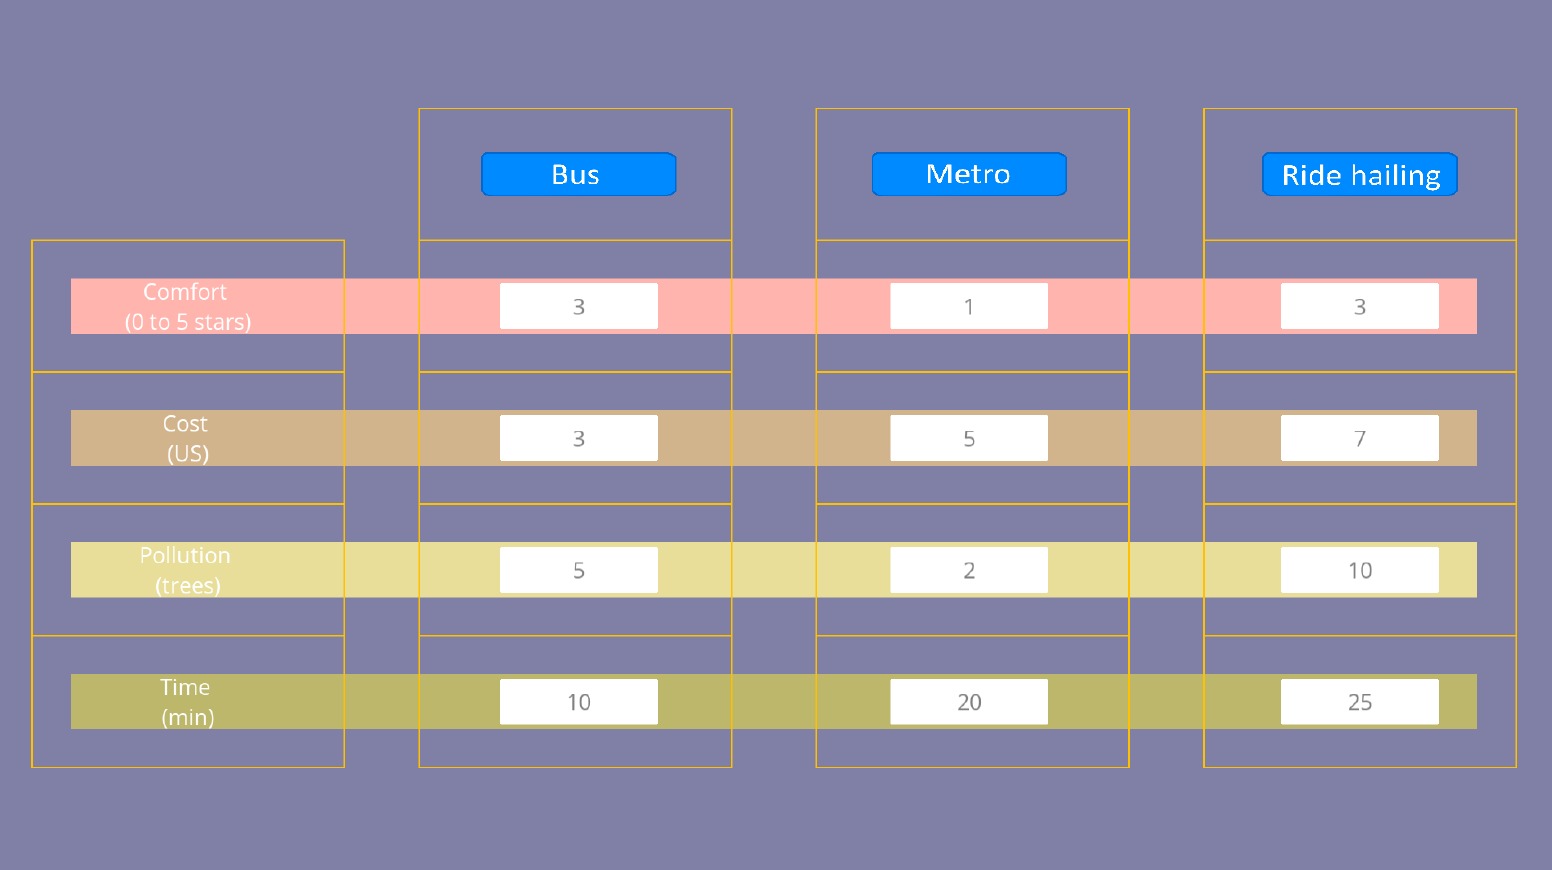
\includegraphics[width=6.33084in,height=3.55313in]{fig/word_media/media/image2.png}

\emph{Figure X.} \textbf{Regions of interest (ROIs).} For data analysis, the choice screen was divided into 19 ROIs. The analysis included merging the attribute labels in one ROI, the option labels in another and the different vertical and horizontal areas spanning the whole grid to assess the dwell times participants spent attending to each attribute and option, respectively.

\section{Discussion}\label{discussion}

In this experiment, we tested the idea that attention to attributes of different options may not be a static phenomenon, but rather flexible and prone to be affected by manipulations of the decision environment.

To our knowledge, there has been only one study looking into potential parallel mechanisms of attention in encoding different aspects of outcome value, similar to what we explored in this paper. Using eye-tracking, \href{https://www.zotero.org/google-docs/?jIZ3Fc}{(Pool et al., 2019)} presented hungry human participants with stimuli that predicted a food outcome. The position of the outcome in each trial was probabilistic, with some stimuli signaling with higher probability the location of the screen where the outcome would be delivered. In this way, participants had to attend to the stimuli and the outcome in each trial to track the stimulus-outcome contingencies. They then devalued the outcome by satiating subjects on one of the foods and tested the effects on the gaze approach to the outcome locations. Pool et al. found that in spite of the devaluation of the outcome, participants still directed their gaze to the location where the now-devalued outcome was more likely to be delivered , indicating a habit-like behavior of gaze in their experiment. However, when studying pupil dilation after devaluation, they found that pupil dilation was still sensitive to outcome value, suggesting a dissociation between habit-like behavior of gaze approach and pupil dilation as two different mechanisms.

Although Pool et al. employed a Pavlovian task where subjects were passively observing the relationship between events in the experiment, their findings can be paralleled with ours.

By integrating insights from psychology, neuroscience with experimental methods from economics, marketing and engineering, our results provide a new perspective on the cognitive mechanisms underlying habits, offering empirical support for the idea that attention is not merely a passive filter but an active driver of behavioral automation.

\subsubsection{Methods}\label{methods}

Upon arrival, participants completed a calibration procedure using Tobii Pro Spark eye-tracking devices under controlled lighting conditions. They were instructed to avoid head movement, remain focused on the screen, and imagine commuting to work during the task. The experiment was implemented in PsychoPy and run on Acer TravelMate P215-54 laptops in NeuroLab (Universidad de Chile). After completing the experiment, participants filled out a brief demographic questionnaire.

\subsubsection{Stimuli and Experimental Setup}\label{stimuli-and-experimental-setup}

All attribute levels were integer values. The choice sets were generated by fully combining attribute levels and optimizing them using the ChoiceDesign Python package to ensure balance, minimize dominated alternatives, and avoid trivial decisions. The design was intended to promote active information processing and support the detection of habit-like behavior through attention narrowing.

Figure 1 displays the interface layout, including regions of interest used for eye-tracking analysis.

\subsubsection{Eye-Tracking and Measures}\label{eye-tracking-and-measures}

Eye-tracking data were collected throughout all trials. For each trial, the following measures were recorded:

\begin{itemize}
\item
  Participant ID and trial number
\item
  Response time
\item
  Chosen option
\item
  Attribute values per option
\item
  Screen coordinates of attribute labels, options, and values
\item
  Fixation durations (in seconds) per element
\item
  Pupil diameter (per frame)
\end{itemize}

Fixation durations were computed by summing all gaze events within predefined areas of interest (ROIs), as shown in Figure 2. Trials with invalid timestamps (e.g., negative durations) were excluded. A total of 5,848 valid trials were included in the final dataset.

\subsubsection{}\label{section-2}

Sebastián's Part

Methodology

Introduction

The experiment was realized with 39 participants, mostly from Universidad de Chile, where they completed a series of 150 tasks of choices between three transport alternatives with different attributes as cost, time travel, comfort and pollution.

The order of the alternatives was fixed, and there were 2 sessions in the process:

\begin{itemize}
\item
  Training: which consisted of 100 tasks, designed to automate the behavior of the participant. The order of the attributes is randomized per participant, and fixed in the whole session.
\item
  Manipulation: consisted in 50 tasks, where the order of the attributes presented switched every 5 tasks. It\textquotesingle s purpose is to recapture attention.
\end{itemize}

For the data acquisition eye-trackers Tobii Pro Spark were used, recording the eye movements from the participants during a task. This lets quantify how many seconds were invested per element in the experiment, including the labels and values presented.

The experiment ran in computers ACER TravelMate P215-54 using Python\textquotesingle s library PsychoPy. THe values of the attributes from the transports were generated combining discrete values, and were optimized later on using a Python\textquotesingle s package called ChoiceDesign, in order to reduce dominant strategies in order to exhaust the participant and that way, automate faster their behavior.

Before the experiment, the participants were given some instructions, asked about their energy levels and how to realize the experiment, as what they were allowed and not to do during the process. Using the eye-tracker driver, the Tobiis were calibrated.

\section{\texorpdfstring{ Preregistration Statement}{ Preregistration Statement}}\label{preregistration-statement}

This study was not preregistered.

\section{Author note}\label{author-note}

Omar David Perez is supported by Instituto de Sistemas Complejos de Ingeniería (ISCI) ANID PIA/PUENTE AFB220002, ANID-SIA 85220023 and ANID-FONDECYT 1231027.

\section{Author contributions}\label{author-contributions}

ODP and BH designed the study. SM programmed the tasks and conducted the experiments. SM and BH analyzed the data. ODP drafted the manuscript, with critical editions by all authors.

Models

\textbf{Preference and Attention Correlation (PAC) models}

The second question is regarding the evolution of preferences over time and after the manipulation. For that, we estimated a MNL to capture preferences heterogeineity intrasubjects, using the fixation time of each attribute as a proxy of the level of attention. If preferences for attributes are correlated with attention, then we should find a significant effect of fixation time over the preferences parameters. This correlation is not claiming any necessary correlation, i.e, the underlying mechanism may be either top-down or bottom-up. We refer to this phenomena as preferences and attention correlation (PAC).

This section describes the main model used for the following analysis. We compared this model with three constrained versions, to show the improvement in model fit caused by the inclusion of visual attention data and intraindividual heterogeneity in preferences parameters.

The utility (\(U_{it}\)) a subject perceives for an alternative \(i\) on a trial \(t\) of the experiment is given by:

\(U_{it} = \sum_{k}^{}{\widehat{\beta}}_{kt}x_{kit}\  + \eta_{it}\ \)

where \({\widehat{\beta}}_{k}\) is the preference parameter of an attribute \(k\) on trial \(t\), and \(x_{kit}\) is the value of the attribute for alternative \(i\). The error term \(\eta_{it}\) is an error term with assumed Gumbel distribution, that captures unobserved factors that may influence the utility. Note that, for simplicity, we dropped the individual specific index.

To capture intraindividual preferences heterogeneity, we formulate the main model (Mix-PAC), which is a mixed MNL that assumes \({\widehat{\beta}}_{k}\) depends on the time, the manipulation, and fixation time. We compare this model with three constrained specifications. The Mix-T model assumes \({\widehat{\beta}}_{k}\) depends only on time and the manipulation, the Mix model just adds an intraindividual error term, and the MNL model only neglects intraindividual and temporal heterogeneity and is used as a baseline model for this comparison. The specifications are detailed below:

\textbf{Mix-PAC (}\({\widehat{\beta}}_{k} = f(attention,\ time)\)) \textbf{:}

\({\widehat{\beta}}_{inertia} = f(time)\)

\(y_{t\ i} = 1,\ if\ ith\ alternative\ chosen\ on\ trial\ t,\ 0\ otherwise\)

\(U_{ti} = f({\widehat{(\beta}}_{inertia}{+ {\widehat{\beta}}_{time}t)y}_{t - 1,\ i})\)

\({\widehat{\beta}}_{k} = \beta_{k\ } + {\beta_{k}}^{post}\delta_{t,\ post} + ({\beta_{k}}^{time,pre} + {\beta_{k}}^{time,post}\delta_{t,\ post})time_{t\ }\  + ({{\alpha_{k}}^{pre}}^{} + {\alpha_{k}}^{\ post}\delta_{t,\ post}) \cdot F_{k,t}\  + \varepsilon_{k,t\ }\)

\textbf{Mix-T}

\({\widehat{\beta}}_{k} = \beta_{k\ } + {\beta_{k}}^{post}\delta_{t,\ post} + ({\beta_{k}}^{time,pre} + {\beta_{k}}^{time,post}\delta_{t,\ post})time_{t\ }\  + \varepsilon_{k,t\ }\)

\textbf{Mix}

\({\widehat{\beta}}_{k} = \beta_{k\ } + \varepsilon_{k,t\ }\)

\textbf{MNL}

\({\widehat{\beta}}_{k} = \beta_{k\ }\)

where \(\beta_{k\ }\)is an attribute-specific constant and represents the average value of the parameter; \({\beta_{k}}^{post}\) is the fixed effect caused by the manipulation; \({\beta_{k}}^{time,pre}\) is the effect of time before the manipulation and \({\beta_{k}}^{time,post}\) is the effect of time after the manipulation; \({\alpha_{k}}^{pre}\) is the effect of fixation time before the manipulation and \({\alpha_{k}}^{post}\ \)is the effect of fixation time after the manipulation. The dummy variable \(\delta_{t,\ post}\) equals 1 if the trial \(t > 100\), and is 0 if \(t \leq 100\). Finally, \(\varepsilon_{k,t\ }\) represents a random intraindividual error term, with a distribution \(N(0,\sigma_{k})\).

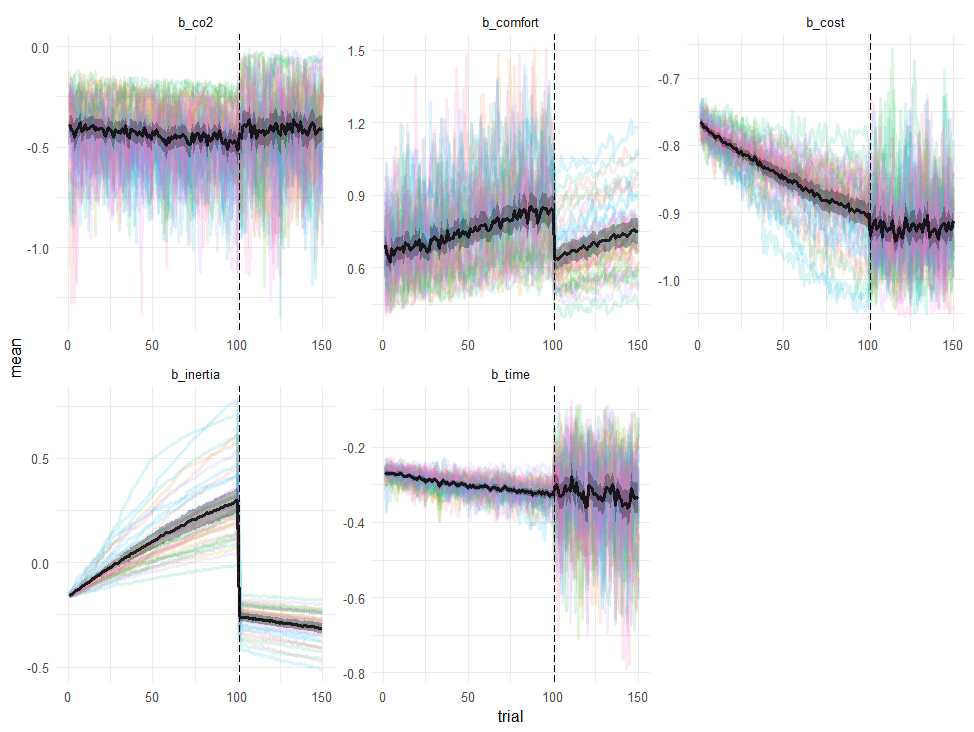
\includegraphics[width=7in,height=5.26389in]{fig/word_media/media/image3.png}

\textbf{Figure X.} \emph{Evolution of attribute weight parameters and inertia over time.} Panels show mean estimated coefficients (black lines with shaded confidence bands) for each attribute and inertia across trials, overlaid with individual trajectories (colored lines). Before the manipulation (trials 1--100), the model reveals a progressive increase in \emph{inertia} (bottom left) and a strengthening of the weight assigned to \emph{cost} (top right), suggesting a growing reliance on repeated prior choices and on that specific attribute. After the manipulation (trial \textgreater{} 100), inertia drops sharply, and attention-weighted coefficients become more stable across participants. Notably, \emph{comfort} and \emph{CO₂} regain some influence post-manipulation, while \emph{time} shows a subtle but consistent trajectory. The attribute \emph{comfort}---which initially played a modest role---became increasingly influential, particularly after the manipulation, indicating that changes in attentional deployment may restore consideration of previously neglected attributes.

\section{}\label{section-3}

\section{}\label{section-4}

\section{}\label{section-5}

\section{}\label{section-6}

\section{References}\label{references}

\href{https://www.zotero.org/google-docs/?BlKSSL}{Adams, C. D., \& Dickinson, A. (1981). Instrumental responding following reinforcer devaluation. \emph{The Quarterly Journal of Experimental Psychology Section B\,: Comparative and Physiological Psychology}, \emph{33}(2), 109--121. https://doi.org/10.1080/14640748108400816}

\href{https://www.zotero.org/google-docs/?BlKSSL}{Bouton, M. E. (2024). Situating Habit and Goal-Direction in a General View of Instrumental Behavior. In Y. Vandaele (Ed.), \emph{Habits} (pp. 45--67). Springer International Publishing. https://doi.org/10.1007/978-3-031-55889-4\_3}

\href{https://www.zotero.org/google-docs/?BlKSSL}{Bouton, M. E., Broomer, M. C., Rey, C. N., \& Thrailkill, E. A. (2020). Unexpected food outcomes can return a habit to goal-directed action. \emph{Neurobiology of Learning and Memory}, 107163.}

\href{https://www.zotero.org/google-docs/?BlKSSL}{Daw, N. D., Niv, Y., \& Dayan, P. (2005). Uncertainty-based competition between prefrontal and dorsolateral striatal systems for behavioral control. \emph{Nature Neuroscience}, \emph{8}(12), 1704--1711. https://doi.org/10.1038/nn1560}

\href{https://www.zotero.org/google-docs/?BlKSSL}{Dayan, P., Kakade, S., \& Montague, P. R. (2000). Learning and selective attention. \emph{Nature Neuroscience}, \emph{3 Suppl}(november), 1218--1223. https://doi.org/10.1038/81504}

\href{https://www.zotero.org/google-docs/?BlKSSL}{Dickinson, A. (1985). Actions and habits: The development of behavioural autonomy. \emph{Philosophical Transactions of the Royal Society B: Biological Sciences}, \emph{308}(1135), 67--78.}

\href{https://www.zotero.org/google-docs/?BlKSSL}{Dolan, R. J., \& Dayan, P. (2013). Goals and habits in the brain. \emph{Neuron}, \emph{80}(2), 312--325. https://doi.org/10.1016/j.neuron.2013.09.007}

\href{https://www.zotero.org/google-docs/?BlKSSL}{Gottlieb, J. (2012). Attention, Learning, and the Value of Information. \emph{Neuron}, \emph{76}(2), 281--295. https://doi.org/10.1016/j.neuron.2012.09.034}

\href{https://www.zotero.org/google-docs/?BlKSSL}{Hardwick, R. M., Forrence, A. D., Krakauer, J. W., \& Haith, A. M. (2019). Time-dependent competition between goal-directed and habitual response preparation. \emph{Nature Human Behaviour}, \emph{3}(12), 1252--1262. https://doi.org/10.1038/s41562-019-0725-0}

\href{https://www.zotero.org/google-docs/?BlKSSL}{Larcom, S., Rauch, F., \& Willems, T. (2017). The benefits of forced experimentation: Striking evidence from the London underground network. \emph{The Quarterly Journal of Economics}, \emph{132}(4), 2019--2055.}

\href{https://www.zotero.org/google-docs/?BlKSSL}{Lee, S. W., Shimojo, S., \& O'Doherty, J. P. (2014). Neural computations underlying arbitration between model-based and model-free learning. \emph{Neuron}, \emph{81}(3), 687--699. https://doi.org/10.1016/j.neuron.2013.11.028}

\href{https://www.zotero.org/google-docs/?BlKSSL}{Perez, O. D., \& Dickinson, A. (2020). A Theory of Actions and Habits: The Interaction of Rate Correlation and Contiguity Systems in Free-Operant Behavior. \emph{Psychological Review}. https://doi.org/10.1037/rev0000201}

\href{https://www.zotero.org/google-docs/?BlKSSL}{Pool, E. R., Gera, R., Fransen, A., Perez, O. D., Cremer, A., Aleksic, M., Tanwisuth, S., Quail, S., Ceceli, A. O., \& Manfredi, D. A. (2022). Determining the effects of training duration on the behavioral expression of habitual control in humans: A multilaboratory investigation. \emph{Learning \& Memory}, \emph{29}(1), 16--28.}

\href{https://www.zotero.org/google-docs/?BlKSSL}{Pool, E. R., Pauli, W. M., Kress, C. S., \& O'Doherty, J. (2019). Behavioural evidence for parallel outcome-sensitive and outcome-insensitive Pavlovian learning systems in humans. \emph{Nature Human Behaviour}, \emph{3}(March). https://doi.org/10.1038/s41562-018-0527-9}

\href{https://www.zotero.org/google-docs/?BlKSSL}{RStudio Team. (2020). \emph{RStudio: Integrated Development Environment for R}. RStudio, PBC. http://www.rstudio.com/}

\href{https://www.zotero.org/google-docs/?BlKSSL}{Thrailkill, E. A., Trask, S., Vidal, P., Alcalá, J. A., \& Bouton, M. E. (2018). \emph{Stimulus Control of Actions and Habits: A Role for Reinforcer Predictability and Attention in the Development of Habitual Behavior}. \emph{44}(4), 370--384.}

\textbf{Appendix}

\textbf{Attributes Non Attendance (ANA) model}

The first question is regarding the evolution of attention over time and the effect of the manipulation in attention. Despite statistical analysis of eye-tracking data sheds light on the changes that the decision-making mechanism may have suffered during the experiment, it does not link properly the relationship between visually attended attributes and the choices made by individuals.

The phenomena of ignoring attributes in discrete choice situations is known as Attributes non Attendance (ANA). In this paradigm, attention is understood as gathering information of an attribute and considering it in decision making. This can be modelled assuming the individual will, stochastically, attend a subset of the available attributes. Then, if there is a set of attributes \(A\), there is a subset of attributes \(A' \in A\) which is actually attended by the individual. This set of attended attributes is the \emph{attention pattern}. Then, \(A'_{t}\) will denote the attention pattern at a given time, assuming each individual\textquotesingle s attention pattern is heterogenous over time.

Then the utility of each alternative \(i\) for a given time instant \(t\) can be specified as \(U_{it} = U(\beta_{k,\ }x_{kit}),\ k \in A'_{t}\ \). Note that, if \(K = |A|\), there are \(2^{K}\) possible subsets, which are all the possible combinations of attention patterns.

We will adapt the ANA model, proposed by Hole et al. (2011). In later formulation, Yegoryan et al. (2020) showed an improved performance of the model after including average measures of fixations. This has the limitation that they assume no evolution of the attention pattern over the experiment, which may be a valid assumption for typical short experiments (e.g. 10 choice tasks). However, this assumption is questionable in long-repeated-choices experiments.

First, let us assume there is a systematic utility \(V_{kt}\) associated with each attribute, which modules the probability of attending that attribute. This utility is a function of time (\(time_{t}\)), the manipulation (\(\delta_{t,\ post} = 1\) if \(t > 100\), and 0 otherwise), and visual attention (fixation time, \(F_{k,t}\ \)):

\(V_{kt} = \gamma_{k\ } + {\gamma_{k}}^{post}\delta_{t,\ post} + ({\gamma_{k}}^{time,pre} + {\gamma_{k}}^{time,post}\delta_{t,\ post})time_{t\ }\  + ({{\gamma_{k}}^{va,\ pre}}^{} + {\gamma_{k}}^{\ va,\ post}\delta_{t,\ post}) \cdot F_{k,t}\ \)

The individual may attend or not each attribute, which generates a binary situation, where the probability \(\pi_{kt}\) of attending an attribute \(k\) is given by:

\({\pi_{kt} = \frac{exp(V_{kt})}{1 + exp(V_{kt})}\ \ }_{}\ \)

Then, the join probability of attending all the attributes in a subset \(A' \in A\), is given by \(\tau(A'):\)

\(\tau(A') = \prod_{k \in A'}^{}\pi_{kt} = \prod_{k \in A}^{}{\pi_{kt}}^{{\lambda_{k}}^{A'}}(1 - \pi_{kt})^{1 - {\lambda_{k}}^{A'}},\ {\lambda_{k}}^{A'} = 1\ if\ k \in A',\ and\ 0\ in\ other\ case\)

Then, let us specify the utility \(V_{itA'}\) of each alternative \(i\), as a function of the attributes in the subset \(A'\):

\(V_{itA'} = \sum_{k \in A'}^{}\beta_{kt}x_{kit}\),

with \(\beta_{kt}\) parameters and \(x_{kit}\) attributes. The conditional probability of choosing an alternative given by:

\(P(y_{it} = 1|A') = \frac{exp(V_{itA'})}{\sum_{j \in A'}^{}exp(V_{jtA'})}\),

where \(y_{it}\) is an indicator function that equals 1 if the subject chooses the alternative \(i\) and 0 if not.

Then, the expected value of the probability of choosing the alternative \(i\), can be calculated by taking the product of the conditional probability and the probability of attending each subset of attributes.

\(P(y_{it} = 1) = \sum_{A' \in A}^{}P(y_{it} = 1|A')\tau(A')\)
